\section{MEAN}

\paragraph{Spørgsmål}
Redegøre for principperne for webudvikling i et server-side MVC framework, og vigtigste karakteristika i et server-side	MVC framework til webudvikling med udgangspunkt i MEAN stacken. Samt vis hvordan man kan designe og implementere en	webløsning, som omfatter persistering af data i en database med anvendelse af MongoDb.

\subsection{MEAN Stack}
Gratis og open-source javascript software stack til udvikling af dynamiske webapplikation. Indeholder følgende elementer:

\paragraph{MongoDB} Dokument-orienteret database system. Klassificeret som NoSQL. Giver mulighed for sharding og automatisk replikation af data.

\paragraph{Express.js} Webapplikations framework til Node. Lightweight med mange features som plugins. Står for routing og middelware.

\paragraph{Angular} Front-end framework udviklet af Google. Bruges til at lave modulære single-page applikationer.

\paragraph{Node.js} Run-time javascript miljø til at eksekvere javascript kode server-side. Hurtig event-dreven arkitektur som tilgodeser throughput og skalering.

\subsection{MVC}
Figur~\ref{fig:mean-mvc} viser hvordan Express.js er tilpasset MVC ved brug af controller klasse.

\begin{figure}[h]
	\centering
	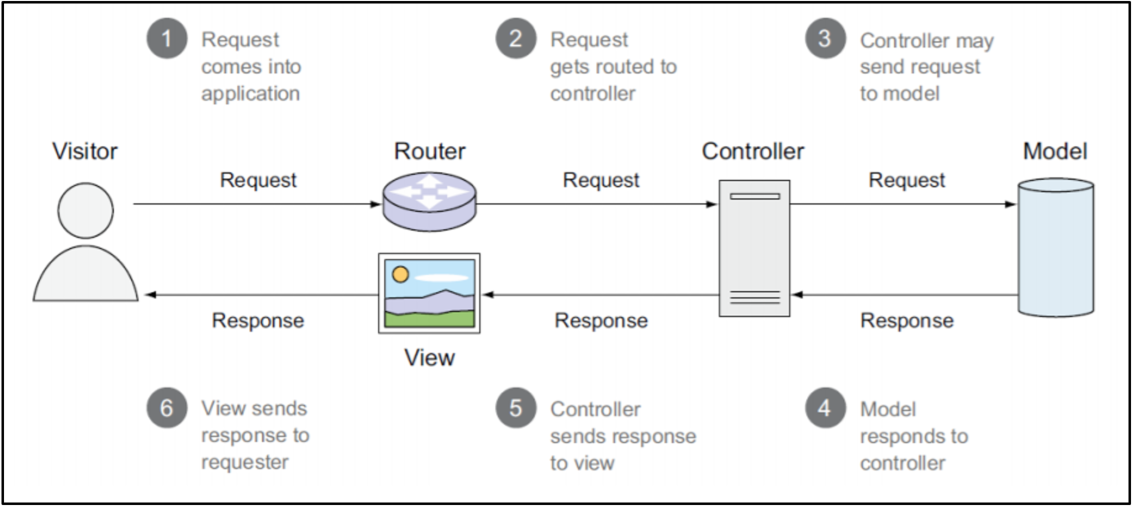
\includegraphics[width=\linewidth]{figs/spm2/mean-mvc}
	\caption{Tilpasning af express.js til MVC.}
	\label{fig:mean-mvc}
\end{figure}
